\let\lesson\undefined
\newcommand{\lesson}{\phantomlesson{Bài 13.}}
\setcounter{section}{2}
\section{Trắc nghiệm nhiều phương án lựa chọn}
\setcounter{ex}{0}
\Opensolutionfile{ans}[ans/VN10-Y24-PH-SYL-022P-TN]
% ===================================================================
\begin{ex}\mkstar{1}
	Hợp lực của hai lực song song cùng chiều là một lực song song
	\choice
	{\True cùng chiều, có độ lớn bằng tổng độ lớn hai lực thành phần}
	{cùng chiều, có độ lớn bằng hiệu độ lớn hai lực thành phần}
	{ngược chiều, có độ lớn bằng tổng độ lớn hai lực thành phần}
	{ngược chiều, có độ lớn bằng hiệu độ lớn hai lực thành phần}
	\loigiai{Hợp lực của hai lực song song cùng chiều là một lực song song cùng chiều, có độ lớn bằng tổng độ lớn hai lực thành phần.}
\end{ex}
% ===================================================================
\begin{ex}\mkstar{1}
	Nhận xét nào sau đây về hợp lực của hai lực song song cùng chiều là \textbf{không đúng}?
	\choice
	{Độ lớn của hợp lực bằng tổng độ lớn của hai lực thành phần}
	{Hợp lực có hướng cùng chiều với chiều của hai lực thành phần}
	{\True Hợp lực có giá nằm trong khoảng cách giữa hai giá của hai lực thành phần và chia thành những đoạn tỉ lệ thuận với độ lớn của hai lực ấy}
	{Điểm đặt của hợp lực chia khoảng cách giữa hai giá của hai lực thành phần thành $d_1$ và $d_2$ thì ta có hệ thức: $\dfrac{F_1}{d_2}=\dfrac{F_2}{d_1}$}
	\loigiai{Hợp lực có giá nằm trong khoảng cách giữa hai giá của hai lực thành phần và chia thành những đoạn tỉ lệ  nghịch với độ lớn của hai lực ấy:
		$$\dfrac{d_1}{d_2}=\dfrac{F_2}{F_1}.$$}
\end{ex}
% ===================================================================
\begin{ex}\mkstar{1}
Hai lực song song cùng chiều có độ lớn lần lượt là $F_1$ và $F_2$ với $F_2>F_1$, lực tổng hợp của hai lực đó có độ lớn là $F$ thì	
	\choice
	{$F=\left|F_1-F_2\right|$}
	{$F=\dfrac{F_1+F_2}{2}$}
	{$F=\sqrt{F_1F_2}$}
	{\True $F=F_1+F_2$}
	\loigiai{}
\end{ex}
% ===================================================================
\begin{ex}\mkstar{2}
	Hai lực $\vec{F}_1$ và $\vec{F}_2$, song song, cùng chiều lần lượt đặt vuông góc tại hai đầu thanh AB có chiều dài $\SI{40}{\centi\meter}$. Biết $F_1=\SI{8}{\newton}$ và $F_2=\SI{12}{\newton}$. Hợp lực $\vec F$ đặt tại O cách A một đoạn là
	\choice
	{$\SI{12}{\centi\meter}$}
	{$\SI{16}{\centi\meter}$}
	{\True $\SI{24}{\centi\meter}$}
	{$\SI{30}{\centi\meter}$}
	\loigiai{Áp dụng quy tắc tổng hợp hai lực song song cùng chiều:
		$$\dfrac{OA}{OB}=\dfrac{F_2}{F_1}=\dfrac{\SI{12}{\newton}}{\SI{8}{\newton}}=\dfrac{3}{2}$$
		Mà $OA+OB=AB=\SI{40}{\centi\meter}$
		Nên:
		\begin{align*}
			\begin{cases}
				OA=\frac{3}{5}\cdot AB=\SI{24}{\centi\meter}\\
				OB=\frac{2}{5}\cdot AB=\SI{16}{\centi\meter}
			\end{cases}
	\end{align*}}
\end{ex}
% ===================================================================
\begin{ex}\mkstar{2}
	Đặt tại hai đầu thanh AB dài $\SI{40}{\centi\meter}$ hai lực song song cùng chiều và vuông góc với AB. Hợp lực $\vec{F}$ đặt tại O cách A một đoạn $\SI{25}{\centi\meter}$ và có độ lớn bằng $\SI{10}{\newton}$. Độ lớn của $\vec{F}_1$ đặt tại A bằng
	\choice
	{$\SI{2.25}{\newton}$}
	{$\SI{8.25}{\newton}$}
	{\True $\SI{3.75}{\newton}$}
	{$\SI{6.25}{\newton}$}
	\loigiai{
	Áp dụng quy tắc tổng hợp hai lực song song cùng chiều:
	$$\begin{cases}
		F_1+F_2=\SI{10}{\newton}\\
		\dfrac{F_1}{F_2}=\dfrac{d_2}{d_1}=\dfrac{15}{25}
	\end{cases}\Rightarrow \begin{cases}
	F_1=\SI{3.75}{\newton}\\
	F_2=\SI{6.25}{\newton}
	\end{cases}.$$
	}
\end{ex}
% ===================================================================
\begin{ex}\mkstar{2}
	Trong bài hát "\textbf{Gánh con gánh cả cuộc đời}" của tác giả Đình Văn có câu: \textit{"Ngày xưa mẹ tôi gánh rau, ra bán chợ huyện xã, một bên gánh rau một bên gánh con, cả cuộc đời dãi nắng dầm mưa".} Ta dễ dàng bắt gặp hình ảnh một người mẹ xưa vất vả, vừa gánh con vừa gánh hàng ra chợ bán như hình.
	\begin{center}
		
\includegraphics[width=0.3\linewidth]{../figs/VN10-2023-PH-TP022-P-2}
	\end{center}
	 Xem đòn gánh là một thanh nhẹ, đồng chất, tiết diện đều, dài $\SI{2}{\meter}$. Em bé có khối lượng $\SI{10}{\kilogram}$ và hàng có khối lượng $\SI{15}{\kilogram}$ đặt ở hai đầu của đòn gánh. Bỏ qua khối lượng của quang gánh. Lấy $g=\SI{10}{\meter/\second^2}$. Người mẹ đặt vai cách phía em bé một khoảng bao nhiêu để cho đòn gánh nằm cân bằng?
	\choice
	{$\SI{0.5}{\meter}$}
	{$\SI{0.8}{\meter}$}
	{$\SI{1.6}{\meter}$}
	{\True $\SI{1.2}{\meter}$}
	\loigiai{
	Ta có:
	\begin{equation}
		\label{eq:1}\\
		d_1+d_2=\SI{2}{\meter}
	\end{equation}
	Áp dụng quy tắc tổng hợp hai lực song song cùng chiều:
	\begin{equation}
		\label{eq:2}\\
		\dfrac{d_1}{d_2}=\dfrac{m_2}{m_1}=1,5
	\end{equation}
	Từ \eqref{eq:1} và \eqref{eq:2}, thu được: $\begin{cases}
		d_1=\SI{1.2}{\meter}\\
		d_2=\SI{0.8}{\meter}
	\end{cases}$.
	}
\end{ex}
% ===================================================================
\begin{ex}\mkstar{3}
	Hai lực $\vec{F}_1$, $\vec{F}_2$ song song cùng chiều theo thứ tự đặt tại hai đầu A và B của thanh AB và vuông góc với thanh. Hợp lực $\vec{F}$ đặt tại O cách A một đoạn $\SI{24}{\centi\meter}$ và cách B đoạn $\SI{16}{\centi\meter}$. Tỉ số $\dfrac{F}{F_2}$ bằng
	\choice
	{$\dfrac{3}{5}$}
	{$\dfrac{3}{2}$}
	{$\dfrac{2}{3}$}
	{\True $\dfrac{5}{3}$}
	\loigiai{
	Áp dụng quy tắc tổng hợp hai lực song song cùng chiều:
	$$\dfrac{F_1}{F_2}=\dfrac{d_2}{d_1}=\dfrac{16}{24}=\dfrac{2}{3}\Rightarrow F_1=\dfrac{2}{3}F_2$$
	Tỉ số
	$$\dfrac{F}{F_2}=\dfrac{F_1+F_2}{F_2}=\dfrac{5}{3}.$$
	
	}
\end{ex}
% ===================================================================
\begin{ex}\mkstar{3}
	Một thanh ngang có khối lượng $\SI{1}{\kilogram}$, chịu tác dụng của ba lực song song, hướng cùng chiều trọng lực và vuông góc với thanh: $F_1=\SI{20}{\newton}$; $F_3=\SI{30}{\newton}$ đặt ở hai đầu thanh và $F_2=\SI{40}{\newton}$ ở chính giữa thanh. Lấy $g=\SI{10}{\meter/\second^2}$. Độ lớn của hợp lực tác dụng lên thanh bằng
	\choice
	{$\SI{50}{\newton}$}
	{$\SI{80}{\newton}$}
	{\True $\SI{100}{\newton}$}
	{$\SI{120}{\newton}$}
	\loigiai{
	Hợp lực tác dụng lên thanh:
	$$F=F_1+F_2+F_3+P=\SI{100}{\newton}.$$
	}
\end{ex}
\Closesolutionfile{ans}
\section{Trắc nghiệm đúng/sai}
\setcounter{ex}{0}
\Opensolutionfile{ans}[ans/VN10-Y24-PH-SYL-022P-TF]
% ===================================================================
\begin{ex}\mkstar{3}
	Một người dùng đòn gánh dài $\SI{1.8}{\meter}$ để gánh hai vật $m_1=\SI{20}{\kilogram}$ và $m_2=\SI{25}{\kilogram}$ như hình vẽ. 
	\begin{center}
		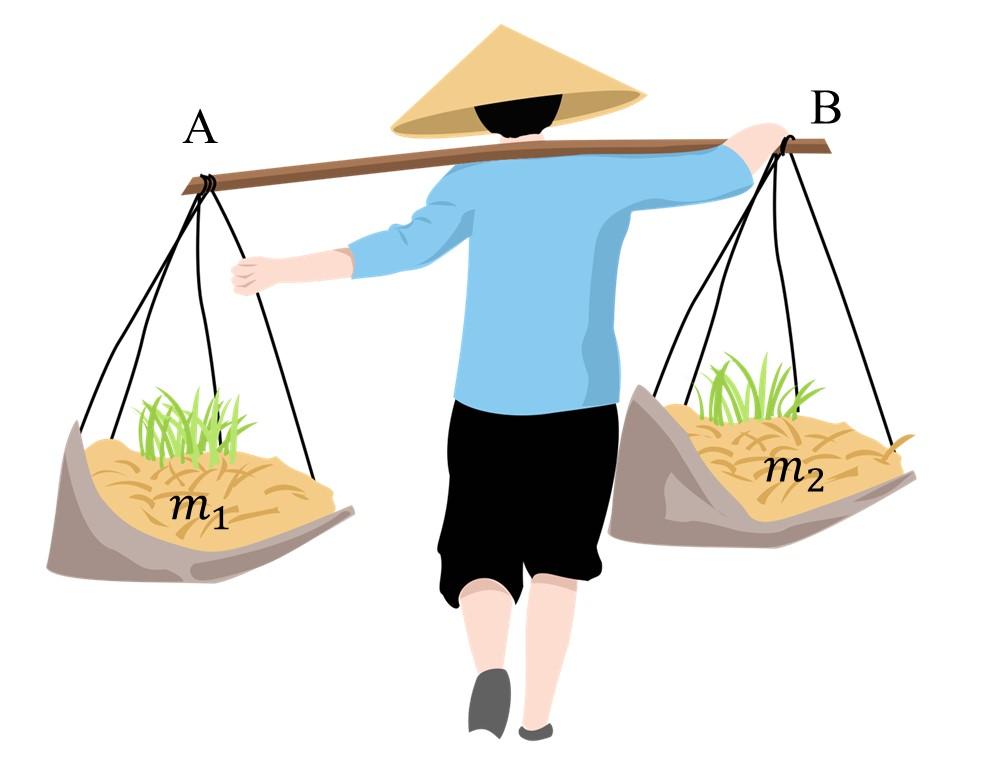
\includegraphics[width=0.3\linewidth]{../figs/VN10-2023-PH-TP022-P-1}
	\end{center}
	Biết điểm treo hai quang gánh được đặt sát hai đầu đòn gánh, bỏ qua khối lượng của đòn gánh.  Lấy $g=\SI{10}{\meter/\second^2}$.
	\choiceTF[t]
	{Trọng lực của vật $m_1$ tác dụng lên đầu A và trọng lực của vật $m_2$ tác dụng lên đầu B là như nhau}
	{\True Điểm đặt vai của người chịu tác dụng của hai lực song song cùng chiều}
	{Để đòn gánh nằm ngang cân bằng thì vai người đặt ở vị trí chính giữa của đòn gánh}
	{\True Khi gánh nằm ngang thì độ lớn lực của đòn gánh tác dụng lên vai là $\SI{450}{\newton}$ và vai cách đầu A đoạn $\SI{1}{\meter}$}
	\loigiai{
	\begin{itemchoice}
		\itemch Sai. $P_1=\SI{200}{\newton}$; $P_2=\SI{250}{\newton}$.
		\itemch Đúng.
		\itemch Sai. $\dfrac{d_2}{d_1}=\dfrac{P_1}{P_2}=\dfrac{4}{5}$ mà $d_1+d_2=\SI{1.8}{\meter}\Rightarrow \begin{cases}
			d_1=\SI{1}{\meter}\\
			d_2=\SI{0.8}{\meter}
		\end{cases}$.
		\itemch Đúng.
	\end{itemchoice}
	}
\end{ex}
\Closesolutionfile{ans}
\section{Tự luận}
\setcounter{ex}{0}
\Opensolutionfile{ans}[ans/VN10-Y24-PH-SYL-022P-TL]
% ======================================================================
\begin{ex}\mkstar{2}
	Một thanh chắn đường dài $\SI{7.8}{\meter}$ có khối lượng $\SI{210}{\kilogram}$, có trọng tâm ở cách đầu bên trái $\SI{1.2}{\meter}$. Thanh có thể quay quanh một trục nằm ngang ở cách đầu bên trái $\SI{1.5}{\meter}$. Hỏi phải tác dụng vào đầu bên phải một lực có độ lớn bao nhiêu để giữ cho thanh nằm ngang? Lấy $g=\SI{10}{\meter/\second^2}$.
	\loigiai{Áp dụng quy tắc tổng hợp hai lực song song cùng chiều:
		$$\dfrac{F}{P}=\dfrac{d_P}{d_F}=\dfrac{\SI{0.3}{\meter}}{\SI{6.3}{\meter}}=\dfrac{1}{21}\Rightarrow F=\dfrac{P}{21}=\SI{100}{\newton}.$$}
\end{ex}
% ======================================================================
\begin{ex}\mkstar{2}
	Hai người khiêng một thanh dầm bằng gỗ nặng, có chiều dài $L$, tiết diện đều. Người thứ hai khoẻ hơn người thứ nhất. Nếu tay người thứ nhất nâng một đầu thanh thì tay của người thứ hai phải đặt cách đầu kia của thanh một đoạn bằng bao nhiêu để người thứ hai chịu lực lớn gấp đôi người thứ nhất? Giả sử rằng trọng tâm của thanh dầm ở ngay chính giữa thanh.
	\loigiai{Áp dụng quy tắc tổng hợp lực song song cùng chiều:
		$$\dfrac{F_2}{F_1}=\dfrac{d_1}{d_2}=2\Rightarrow d_2=\dfrac{d_1}{2}=\dfrac{L}{4}.$$
		Vậy người thứ hai phải đặt tay cách đầu kia của thanh đoạn $\dfrac{L}{4}$.}
\end{ex}
% ======================================================================
\begin{ex}\mkstar{2}
	Một tấm ván nặng $\SI{240}{\newton}$ được bắc qua một con mương. Trọng tâm của tấm ván cách điểm tựa A đoạn $\SI{2.4}{\meter}$ và cách điểm tựa B đoạn $\SI{1.2}{\meter}$. Hỏi lực mà tấm ván tác dụng lên điểm tựa A một đoạn bằng bao nhiêu?
	\loigiai{Lực do tấm ván đè lên điểm tựa A và B là hai lực song song cùng chiều:
		\begin{equation}
			\label{eq:22.7}
			F_A+F_B=P=\SI{240}{\newton}
		\end{equation}
		Áp dụng quy tắc tổng hợp hai lực song song cùng chiều:
		\begin{equation}
			\label{eq:22.8}
			\dfrac{F_{\mathrm{A}}}{F_{\mathrm{B}}}=\dfrac{d_{\mathrm{B}}}{d_{\mathrm{A}}}\Leftrightarrow \dfrac{F_{\mathrm{A}}}{F_{\mathrm{B}}}=\dfrac{\SI{1.2}{\meter}}{\SI{2.4}{\meter}}=\dfrac{1}{2}
		\end{equation}
		Từ \eqref{eq:22.7} và \eqref{eq:22.8}, suy ra:
		$$F_A=\SI{80}{\newton}, \quad F_B=\SI{160}{\newton}.$$}
\end{ex}
% ======================================================================
\begin{ex}\mkstar{2}
	Một người đang quẩy trên vai một chiếc bị có trọng lượng $\SI{40}{\newton}$. Chiếc bị buộc ở đầu gậy cách vai $\SI{70}{\centi\meter}$, tay người giữ ở đầu kia cách vai $\SI{35}{\centi\meter}$. Bỏ qua trọng lượng của gậy, hỏi lực giữ gậy của tay và vai người sẽ chịu một lực có độ lớn bằng bao nhiêu?
	\loigiai{	Gọi:
		\begin{itemize}
			\item $F_1$, $F_2$ lần lượt là lực do tay tác dụng lên đầu gậy và lực do chiếc bị tác dụng lên đầu gậy.
			\item $d_1$, $d_2$ lần lượt là khoảng cách từ vị trí tay nắm đến vai và khoảng cách từ chiếc bị đến vai.
		\end{itemize}
		Áp dụng quy tắc tổng hợp lực song song cùng chiều:
		$$\dfrac{F_2}{F_1}=\dfrac{d_1}{d_2}\Rightarrow F_1=\dfrac{F_2d_2}{d_1}=\dfrac{\left(\SI{40}{\newton}\right)\cdot\left(\SI{70}{\centi\meter}\right)}{\SI{35}{\centi\meter}}=\SI{80}{\newton}$$
		Lực nén lên vai người:
		$$F=F_1+F_2=\SI{120}{\newton}.$$
	}
\end{ex}
% ======================================================================
\begin{ex}\mkstar{3}
Hai thanh dầm thép đồng chất, có trọng tâm tại A và B, đặt chồng lên nhau như hình \ref{fig:23.8}. Thanh dài hơn có trọng lượng $\SI{10}{\kilo\newton}$.
\begin{center}
	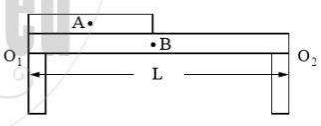
\includegraphics[width=0.4\linewidth]{../figs/VN10-2022-PH-TP022-P-1}
	\captionof{figure}{}
	\label{fig:23.8}
\end{center}
\begin{enumerate}[label=\alph*)]
	\item Xác định hợp lực của trọng lực tác dụng lên hai thanh dầm.
	\item Hai thanh dầm được đặt lên các cột đỡ tại $O_1$ và $O_2$. Để hệ đứng yên thì hợp lực $\vec F$ của các lực đỡ bởi hai cột phải cân bằng với hợp lực $\vec P$ xác định ở câu a. Hỏi mỗi cột đỡ chịu một lực có độ lớn bằng bao nhiêu?
\end{enumerate}	
	\loigiai{\begin{enumerate}[label=\alph*)]
			\item Áp dụng quay tắc hợp lực song song, cùng chiều cho hai trọng lực $\vec P_1$ và $\vec P_2$ của hai thanh, ta xác định được hợp lực $\vec P$:
			\begin{center}
				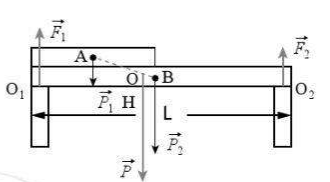
\includegraphics[width=0.4\linewidth]{../figs/VN10-2022-PH-TP022-P-2}
			\end{center}
			\begin{itemize}
				\item Độ lớn $P=P_1+P_2=\SI{15}{\kilo\newton}$.
				\item Giá của $\vec P$ đi qua điểm O chia đoạn AB theo tỉ lệ:
				$$\dfrac{OA}{OB}=\dfrac{P_2}{P_1}=\dfrac{10}{5}=2$$
				Mà khoảng cách giữa giá của $\vec P_1$ và $\vec P_2$ là $\dfrac{L}{4}$ nên khoảng cách từ giá của $\vec P$ đến giá của $\vec P_1$ và $\vec P_2$ lần lượt là $\dfrac{L}{6}$ và $\dfrac{L}{12}$.
			\end{itemize}
			\item Hợp lực $\vec F$ của các lực đỡ bởi hai cột phải cân bằng với $\vec P$, tức là:
			$F=P=\SI{15}{\kilo\newton}$, $\vec F$ ngược chiều và có giá trùng với giá của $\vec P$.\\
			Vì $\vec F$ là hợp lực của hai lực đỡ $\vec F_1$ và $\vec F_2$ song song, cùng chiều nên:
			\begin{align*}
				\begin{cases}
					F_1+F_2=F=\SI{15}{\kilo\newton}\\
					\dfrac{F_1}{F_2}=\dfrac{O_2H}{O_1H}=\dfrac{7}{5}
				\end{cases}
			\end{align*}
			Lực đỡ mỗi cột phải chịu:
			$$F_1=\SI{8.75}{\kilo\newton}; \quad F_2=\SI{6.25}{\kilo\newton}.$$
	\end{enumerate}}
\end{ex}
% ======================================================================
\begin{ex}\mkstar{4}
	Một đĩa tròn phẳng, mỏng, đồng chất, bán kính $R$ sẽ có điểm đặt của trọng lực tại tâm của đĩa. Hỏi khi khoét một lỗ tròn bán kính $\dfrac{R}{2}$ thì trọng tâm của đĩa sẽ ở vị trí nào?
	\begin{center}
		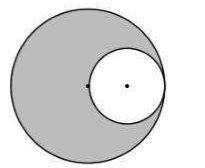
\includegraphics[width=0.2\linewidth]{../figs/VN10-2022-PH-TP022-P-3}
	\end{center}
	\loigiai{Trọng tâm của đĩa bị khoét là điểm đặt hợp lực của trọng lực $P_K$ của hình tròn tâm K bán kính $\dfrac{R}{2}$ và trọng lực $P_I$ của phần đĩa còn lại sau khi khoét đi hai lỗ tròn đối xứng qua I.
		\begin{center}
			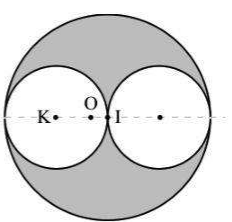
\includegraphics[width=0.2\linewidth]{../figs/VN10-2022-PH-TP022-P-4}
		\end{center}
		Vì đĩa phẳng đồng chất nên trọng lượng mỗi phần đĩa tỉ lệ với diện tích. Gọi $P$ là trọng lượng của đĩa nguyên, ta có:
		$$\dfrac{P_K}{P}=\dfrac{\pi\left(\dfrac{R}{2}\right)^2}{\pi R^2}=\dfrac{1}{4}\Rightarrow P_K=\dfrac{P}{4}$$
		Áp dụng quy tắc tổng hợp lực song song cùng chiều cho các trọng lực $P_I$ và $P_K$, ta xác định được điểm đặt O của hợp lực sẽ chia đoạn IK theo tỉ lệ:
		$$\dfrac{OI}{OK}=\dfrac{P_K}{P_I}=\dfrac{\dfrac{P}{4}}{\dfrac{P}{2}}=\dfrac{1}{2}\Rightarrow OI=\dfrac{R}{6}.$$}
\end{ex}
\Closesolutionfile{ans}
